\documentclass[a4paper,12pt,openright]{report}
\usepackage{libertine}
\usepackage{libertinust1math}
\usepackage[T1]{fontenc}
\usepackage[utf8]{inputenc}
\usepackage[italian]{babel}
\usepackage{lipsum}
%\newcommand{\mostracapitoli}{\includeonly{6_1_cap/1_cap, 6_2_cap/2_cap, 6_3_cap/3_cap, 6_4_cap/4_cap}}
\usepackage{siunitx}
\usepackage{pgfplots}
\usepackage{caption}
\captionsetup{tableposition=top,figureposition=bottom,font=small}
\usepackage[lofdepth,lotdepth]{subfig}
\usepackage{graphicx}
%\usepackage{tabularx}
\usepackage{booktabs}
\usepackage{rotating}
\usepackage{multirow}
\usepackage{longtable}
\usepackage[italian]{varioref}
\sisetup{
		group-digits=true,
		group-separator={.},
		output-decimal-marker={,}
}
\SendSettingsToPgf
%\usepackage{geometry}
\usepackage{quoting}
\quotingsetup{font=small}
\newcommand{\n}[2]{\SI{#1}{#2}}	%comando per valore e unità di misura
%\usepackage{tocloft}RIATTIVA QUESTO
\usepackage[final]{pdfpages} %draft final

%\cftsetindents{chapter}{0em}{2em}RIATTIVA QUESTO
%\cftsetindents{section}{1em}{3em}RIATTIVA QUESTO
%\cftsetindents{subsection}{em}{2em} CERCA DI METTERE IL NUMERO SUBITO DOPO IL TITOLO NELL'INDICE E TOGLI I PUNTINI 

%\renewcommand\cfttoctitlefont{\hfill\Large\bfseries}RIATTIVA QUESTO
%\renewcommand\cftaftertoctitle{\hfill\mbox{}}RIATTIVA QUESTO

%\setcounter{tocdepth}{1} RIATTIVA QUESTO

\newcommand{\uni}{\textbf{Università di Napoli}}
\newcommand{\sdots}{\vspace{0.5em}[\dots]\vspace{0.5em}}
\newcommand{\tit}[2]{{#1}\hspace{0.5mm}{#2}}
\newcommand{\trasm}{\si{W/m^2K}}
\newcommand{\bim}{\textbf{BIM}}
\newcommand{\norvent}{UNI 10339}
\newcommand{\norinv}{UNI EN 12831 (2006)}
\newcommand{\emod}{\textbf{Emodinamica}}
\newcommand{\utic}{\textbf{UTIC}}
\newcommand{\blocc}{\textbf{Blocco Operatorio}}
\newcommand{\corpa}{\textbf{Corpo A}}
\newcommand{\corpc}{\textbf{Corpo C}}
\newcommand{\radd}{\textbf{Radiatori}}
%\mostracapitoli
%\includeonly{6_4_cap/4_cap}
\begin{document}
	\begin{titlepage}
\begin{center}
	\textsc{{\Large
	Università degli Studi di Napoli Federico II\\
	\vspace{0.75em}
	Scuola Politecnica e delle Scienze di Base\\}}
	\vspace{1em}
	{\large\bfseries
	Dipartimento di Ingegneria Industriale\\
	\vspace{0.5em}
	Corso di Laurea in Ingegneria Meccanica\\
	\vspace{0.5em}
	Classe di Laurea L 09\\ }
	\vspace{3em}
	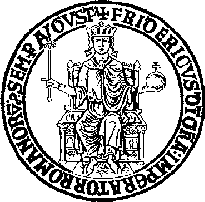
\includegraphics[width=3cm]{0_frontespizio/img/LogoFrontespizio}\\
	\vspace{3em}
	{\Large
	\textsc{ elaborato di laurea in}\\\textsc{riqualificazione energetica di edifici ospedalieri:\vspace{0.2em}\\analisi progettuale relativa all'edificio 2 dell'AOU~"Federico II"}}\\
	\vspace{5em}
	\begin{tabular}{p{8cm}l}
		\textbf{Relatore:}						&	\textbf{Candidato:}\\
		Ch.mo Prof. Ing. Adolfo Palombo 		&	Vincenzo Caccavale\\
		\textbf{Relatore:}						&	M65/646\\
		\tit{Ing.}{Annamaria Buonomano}			& 	\\
		\textbf{Correlatore:}					& 	\\
		\tit{Ing.}{Cesare Forzano}				& 	\\
	\end{tabular}
	\vfill
	Anno Accademico 2016/2017
\end{center}

\end{titlepage}
	\thispagestyle{empty}
\vspace*{1em}
\begin{center}
\large Questa tesi è dedicata a mio padre perché più di tutti nel tempo mi ha rifornito
di quella forza autolesionistica indispensabile per conoscere e continuare a imparare:\\
{\Large\vspace{0.5em} la curiosità}
\end{center}

	\thispagestyle{empty}
\vspace*{1em}
\begin{center}
\large Questa tesi è dedicata a mio padre perché più di tutti nel tempo mi ha rifornito
di quella forza autolesionistica indispensabile per conoscere e continuare a imparare:\\
{\Large\vspace{0.5em} la curiosità}
\end{center}

	\tableofcontents
\thispagestyle{empty}




	SOMMARIO
E IO SO VINCENZO	
	Questa è la pagina per i ringraziamenti.\\ 
dthdd
	\chapter{La prima costruzione del Policlinico}
\thispagestyle{empty}
\addcontentsline{toc}{section}{Il Progetto}
%Si riportano stralci dei primi capitoli del III Volume \textsc{Ospedali e Cliniche Universitarie} dell'Ing. \textsc{Corrado Beguinot}. In questo modo, si spera di riuscire a evidenziare quelle che sono le differenze progettuali tra le normative vigenti all'epoca della costruzione del Policlinico e quelle odierne.\vspace{0.5em}
 
\emph{Con l'inizio dell'anno accademico 1972-73 la seconda Facoltà di Medicina e Chirurgia dell'\uni{} ha \LaTeX{} iniziato la sua attività nella sua nuova sede, all'epoca in parte ultimata ed in parte in corso di ultimazione.}

\emph{Il numero degli studenti supera oggi le \num{6000} unità ed il numero complessivo dei letti è di \num{2758}.}

\emph{La Facoltà è costituita da un organismo edilizio articolato in ventisei edifici nei quali hanno sede gli Istituti, le Cliniche, i servizi e le attrezzature che sono collegati da gallerie di servizio a due livelli e da una viabilità principale e secondaria, e dotati di ampie superfici a verde e di parcheggi. La superficie complessiva su cui è stata realizzata la Facoltà è di \n{440000}{m^2} ed il volume costruito è di \n{11130000}{m^3} con una superficie totale dei piani pari a \n{270000}{m^2}.}

\emph{Il costo dell'opera, comprensivo del costo dei suoli, delle attrezzature didattiche, dell'arredo, delle sistemazioni esterne, degli impianti e degli oneri revisionali, è risultato di circa \num{45} miliardi con un costo quindi a \si{m^3} di \num{40000} lire circa.}

\emph{Gli istituti sono inseriti nei vari edifici in funzione delle loro affinità didattiche e di ricerca ed in funzione della prevista organizzazione dipartimentale.}

\vspace{0.5em}

\noindent Le prime righe di questo elaborato di laurea sono state volutamente lasciate alle parole dell'\tit{ing.}{Corrado Beguinot} il quale coordinò i lavori di progettazione e costruzione del policlinico. 

Inerentemente all'oggetto di questa tesi, ovvero uno studio di riqualificazione energetica dell'involucro e degli impianti annessi dell'Edificio 2 dell'AOU \uni, il Beguinot descrive così l'edificio 2:

\vspace{0.5em}

L'edificio di \emph{Patologia Medica} comprende\emph{: laboratori di ricerca e stabulari per una superficie di circa \n{1200}{m^2}; 1 aula da \num{400} posti, \num{8} aule da \num{30} in comune con la Semeiotica Medica, l'Endocrinologia e la Dermatologia; reparti di degenza per un totale di \num{150} posti-letto, con una superficie di circa \n{4400}{m^2}. La superficie totale dei piani è di \n{8700}{m^2} circa.}

\vspace{0.5em}
\noindent In merito all'involucro opaco e trasparente, l'ingegnere si esprime così:

\vspace{0.5em}

\emph{L'adozione di un sistema modulare generale ha consentito una impostazione unitaria della costruzione dei complessi delle Cliniche, costituiti dai corpi alti delle degenze e dai corpi delle piastre di base degli ambulatori, delle diagnostiche, degli uffici, dei laboratori, delle aule, ecc.}

\emph{La struttura dei corpi di degenza è essenzialmente costituita da una teoria perimetrale di pilastri pressoinflessi, posti ad interasse di \n{1.90}{m}, collegati ai piani da un solaio c.a. realizzato con coppie di travi a sezione rettangolare, agganciate lateralmente ai pilastri, e solette piene in calcestruzzo. La rigidezza globale del sistema è assicurata da una trave perimetrale parapetto e dai blocchi dei collegamenti verticali, scala principale, scale di servizio e di emergenza, costituiti da pareti portanti in c.a. dello spessore di \n{40}{cm}, dalle quali escono a sbalzo i gradini prefabbricati ed i ripiani. Il coronamento dell'edificio è realizzato con elementi modulari prefabbricati in c.a., agganciati al prolungamento dei pilastri.}

\sdots

\emph{Le facciate dei corpi degenza sono caratterizzate, oltre che dagli elementi pieni di calcestruzzo armato dei collegamenti verticali, da una alternanza di pieni e vuoti, realizzati con l'adozione di un elemento tipo prefabbricato, di lunghezza modulare, ancorato mediante piastre, perni e bulloni ai pilastri. I suddetti blocchi sono costituiti da un doppio strato di silicalcite pesante e leggera, e sono rifiniti sulla faccia esterna con una superficie granigliata e sul lato interno a stucco. Lo spazio libero, tra la fascia parapetto e l'intradosso del solaio, è modulato in sette parti uguali, che sono occupate da elementi prefabbricati o elementi di infisso in accordo con le esigenze di visibilità e di illuminazione degli ambienti interni e della composizione della superficie esterna.}

\sdots

\emph{Allo scopo di attenuare la rumorosità negli ambienti sono stati adottati nei corridoi e nelle altre zone di traffico (atrio al piano, soggiorno pazienti, testate di servizio) pavimenti di gomma; nelle camere di degenza, nei soggiorni per i visitatori, e negli studi si è adottata una pavimentazione resiliente. Sia i pavimenti di gomma che quelli resilienti sono posti in opera su sottofondo di arena e cemento. In tutti i locali di servizio, in quelli soggetti a più frequenti lavaggi e disinfezioni, cioè ambienti per la visita medica, laboratori, ecc., si è adottata una pavimentazione in grés opaco.}

\sdots

\emph{Per l'alloggiamento degli impianti sono stati predisposti nelle strutture appositi cavedi, ubicati in posizione tali da servire in maniera omogenea la superficie di ogni piano. Più precisamente sono stati realizzati due grandi cavedi in corrispondenza rispettivamente della scala di sicurezza all'estremità del corpo di fabbrica e del torrino dei servizi, che è anche attraversato verticalmente da altri tre cavedi più piccoli, dei quali due per impianti idrico-sanitari ed uno di forma allungata, riservato esclusivamente agli impianti elettrici. Una serie continua di cavedi attraversa longitudinalmente tutto il corpo della degenza, accogliendo le condotte pluviali, gli scarichi degli impianti idrici annessi alle camere di degenza, le canne di aspirazione delle cappe dei laboratori, nei casi in cui è prevista l'ubicazione di questi ultimi nel piano rialzato del blocco degenza, e le reti di distribuzione dei gas medicali.}

\sdots

\emph{I cavedi, grandi e piccoli, ed ogni altra canalizzazione verticale, al piano cantinato, fanno capo alle reti orizzontali, ospitate nella galleria di servizio.}

\emph{L'isolamento termico delle coperture è ottenuto con l'interposizione, tra solaio ed impermeabilizzazione, di uno strato coibente, sul quale è disposto un masso concreto con pendenza verso l'interno del corpo di fabbrica per il raccordo delle pluviali, sistemate nei cavedi precedentemente descritti.}

\sdots

\emph{Gli infissi esterni sono realizzati con profilo in lamierino di acciaio verniciato a fuoco e vetro semidoppio; quelli delle camere di degenza, alternati con i blocchi di silicalcite, hanno apertura a vasistas e tenda di oscuramento in tessuto plastico; quelli del torrino dei servizi e dell'atrio di piano realizzano una fascia continua verticale, interrotta solo dallo spessore dei solai e dalla fascia parapetto, ed hanno apertura a battente.}

\sdots

\emph{Per quanto riguarda la finitura delle superfici interne ed esterne si ricorda che sono lasciati a vista i getti di calcestruzzo sia all'interno che all'esterno, proteggendoli con vernice idrorepellente ed antipolvere. Le altre pareti ed i soffitti sono dipinti con pittura lavabile. In particolare quelle delle camere di degenza, realizzati, come già detto con solette e travi binate, hanno il calcestruzzo a vista per le travi e l'intradosso delle solette, gettate su cassaforma di compensato marino, semplicemente stuccate e dipinte con pittura lavabile.}

\vspace{0.5em}
\noindent I corpi bassi differiscono di poco dalla struttura modulare di quelli alti. Infatti:

\vspace{0.5em}

\emph{La struttura portante dei corpi bassi conserva la stessa modulazione dei blocchi degenze.}

\sdots

\emph{La trave parete, oltre alla funzione di collegamento e di irrigidimento dell'insieme, ha anche quella di contenimento del terreno per il piano di servizio che corre continuo alle piastre.}

\emph{Le coperture di tali corpi sono realizzate con elementi in cemento armato ad U capovolto, sul modulo tipo di \n{1.90}{m}, poggiati su travi portanti longitudinali, ed uscenti a sbalzo per \n{1.60}{m}, onde realizzare una zona d'ombra sulle pareti verticali.}

\sdots

\emph{Uno strato coibente ed un'impermeabilizzazione a guaina sintetica proteggono le coperture, seguendone il profilo grecato.}

\sdots

\emph{Le facciate esterne sono costituite dall'alternanza di elementi di tompagno e di infissi, suggerita dalla funzionalità esterna.}

\emph{I tompagni sono realizzati con doppia fodera: pannello prefabbricato di cemento granigliato all'esterno, e tavolato di mattoni forati intonacato all'interno. Gli infissi sono in lamiera di acciaio verniciato a fuoco di tipo analogo a quelli del corpo di fabbrica delle degenze.}

Inserisci eventualmente foto prese dal Beguinot o foto dal sopraluogo

Impianto termico e centrale tecnologica a pagina 89


\vspace{1em}
\begin{flushright}
	\textbf{\textsc{Corrado Beguinot}}
\end{flushright}
\newpage
\subsection{aeaefaefaef}
\subsubsection{aefaefaefaefaefa}
	%\chapter{Descrizione del bando}
\thispagestyle{empty}
In attesa\dots NON HO IL BANDO
	\chapter{Descrizione bando}
\thispagestyle{empty}
Vedi al limite di mettere questo capitolo dopo quello riguardante la storia del policlinico.

Prendi degli stralci del bando, sottolineando le parti in cui si specifica la combinazioni di impianti da realizzare. 

Alla fine di questo capitolo metti gli obiettivi della tesi. <-- al limite vedi di inserire questa parte anche nel sommario. Siccome questa parte è introduttiva della tesi (in quanto vengono spiegati gli obiettivi etc etc) vedi di usare questo capitolo come introduttivo o una specie di Introduzione alla tesi prima del primo capitolo vero e proprio.
	\chapter{Lo stato attuale}
\thispagestyle{empty}
\section{Le modifiche al giorno d'oggi}
%Aggiungi un mini indice in questo capitolo se le dimensioni dello stesso iniziano ad essere proibitive.\\
%Parla anche dell'assenza di organi per la misurazione dei consumi (elettrici e termici) e quindi problemi per la valutazione energetica \emph{ante-operam} e per il rispetto ai requisiti \emph{CAM}.\vspace{1em}
Nel primo capitolo si sono descritti in maniera sommaria l'architettura, l'edilizia e gli impianti presenti nell'intero complesso ospedaliero (al momento della costruzione) riportando le parole dell'\tit{ing.}{Corrado Beguinot}. In questo capitolo, invece, si vuole dare ampio spazio alle condizioni attuali del suddetto edificio, riportando i dati di input inseriti all'interno dello studio pre-riqualificazione energetica riferiti, quindi, allo stato di fatto. 

Prima di procedere con suddetto elenco particolareggiato sull'edificio 2, però, si vogliono riportare le modifiche effettuate su tutto l'impianto ospedaliero del policlinico. 

In questi anni, infatti, nella centrale termica, le caldaie vengono fatte funzionare per inviare acqua calda nella rete di teleriscaldamento non più a \n{170}{\degreeCelsius} ma a \n{130}{\degreeCelsius}. Per quanto riguarda il teleriscaldamento.
Il cogeneratore è stato modicato. Sono stati aggiunti questi gruppi frigoriferi di cui tot ad assorbimento.
\clearpage
\section{L'edificio 2}
Tutto il corpo di fabbrica è destinato alla \emph{Cardiochirurgia}.

Esso è costituito da 5 edifici:
\begin{itemize}
	\item Corpo A: è l'edificio principale. Di sviluppo longitudinale lungo un asse orientato lungo la direttrice N-E -- S-O, è alto 5 piani oltre il piano terra. Contiene le degenze, gli ambulatori, l'Emodinamica al piano terra, l'UTIC (Unità di Terapia Intensiva Coronarica) e il blocco operatorio al quinto piano. La sua superficie in pianta è di ... per un totale di ... per i 6 piani.
	\item Corpo B: contiene ... di pianta quadrata ed è alto solo 1 piano. Estensione
	\item Corpo C: contiene laboratori e ambulatori. E' di pianta rettangolare e alto solo 1 piano. Estensione
	\item Corpo D: contiene ... di pianta quadrata ed è alto solo 1 piano. Estensione
	\item Corpo E: contiene ... di pianta quadrata ed è alto solo 1 piano. Estensione
\end{itemize}

I livelli dell'edificio 2 (che sono comunque in comune con quasi tutti gli edifici del Policlinico) sono 8 di cui 2 sotterranei. Infatti, è presente una rete di cunicoli al di sotto del Policlinico che unisce in modo diretto e senza ostacoli (in quanto non è permesso il traffico veicolare al pubblico) i vari edifici. I livelli dei cunicoli sono due: uno è quello \emph{del pulito} (-1) mentre l'altro è quello \emph{dello sporco} (-2).

\textbf{Questa parte mettila dopo aver parlato dell'involucro opaco e trasparente}
Il suddetto edificio è stato suddiviso per questioni di comodità e calcolo in \emph{5~strutture}:
\begin{itemize}
	\item l'\emph{UTIC} è presente al primo piano dell'edificio alto. Comprende le sale operatorie e le relative degenze.
	\item \emph{Emodinamica} situata al piano terra dell'edificio alto. Comprende la sala operatoria, una sala operatoria minore e le relative sale controllo.
	\item il \emph{Quinto Piano} dell'edificio alto. Qui è presente la \emph{Terapia Intensiva}.
	\item il \emph{Corpo Alto} coincide con l'edificio alto escluse le 3 suddette strutture già menzionate. Sono presenti le degenze, le cucine, i servizi e gli uffici.
	\item il \emph{Corpo Basso} collegato a quello alto tramite un doppio tunnel di cui solo uno è oggetto di studio: sono presenti i laboratori di \emph{Patologia Immunitaria}.
\end{itemize}
Si riporta in Fig.~\vref{planimetriapianoterra} la planimetria del Piano Terra con i contorni colorati che evidenziano le zone di intervento. %Ricorda di dire prima perchè ci sono zone di intervento
\begin{sidewaysfigure}
	\centering
	\caption{Planimetria del Piano Terra dell'Edificio 2. Si notino le due aree di intervento.}
	\label{planimetriapianoterra}
	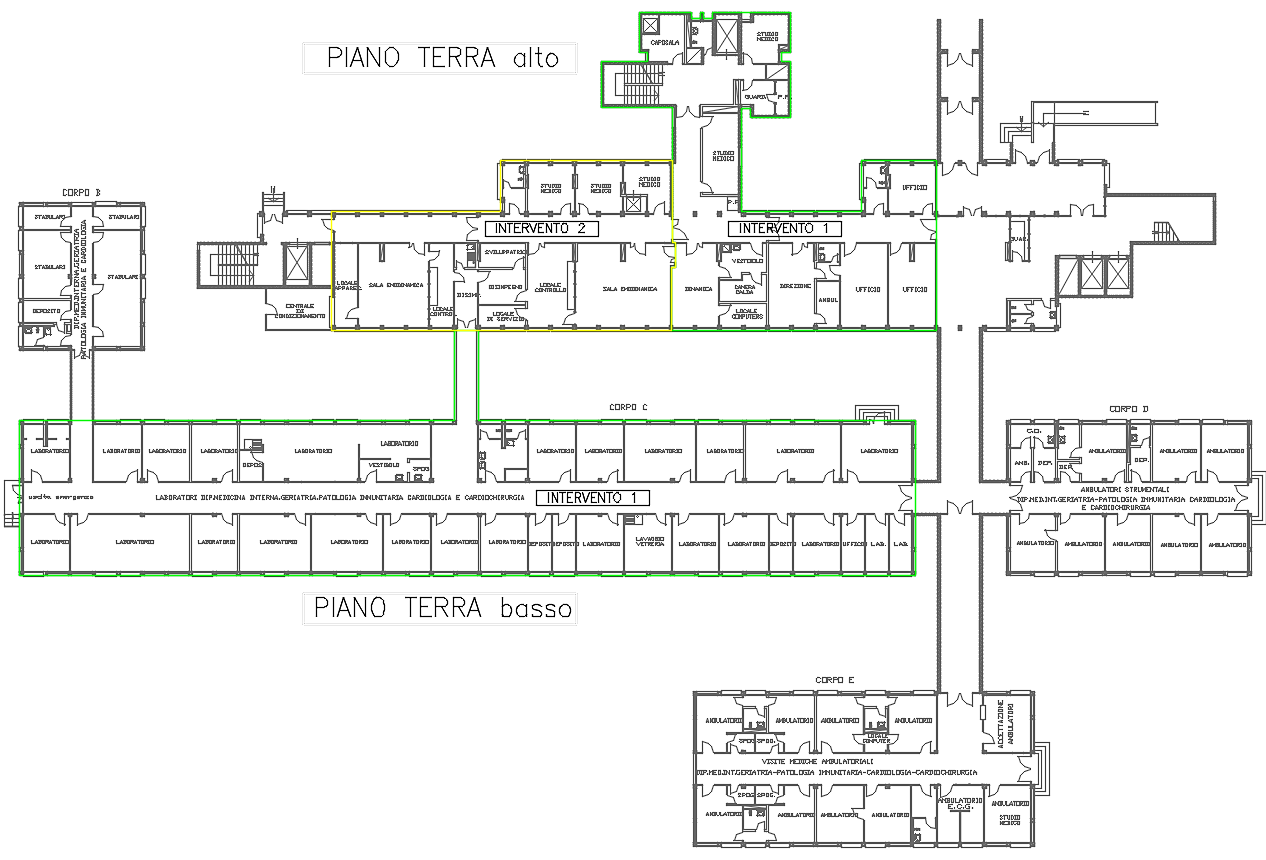
\includegraphics[width=\textheight]{6_2_cap/img/piano_terra}	
\end{sidewaysfigure}

L'edificio 2 preserva tutte le opere edili e impiantistiche realizzate all'epoca della sua costruzione. Non è difficile dedurre, quindi, che allo stato attuale sia i comportamenti estivi e invernali dell'involucro come le efficienze termo-meccaniche dell'impianto idro-aeraulico siano quantomeno inferiori a quelli consigliati dalla norma attuale vigente. 

%\begin{itemize}
%	\item componenti opachi
%	\item componenti trasparenti
%	\item ponti termici???
%	\item definizione dei vari locali
%\end{itemize}
%Metti i risultati con tabelle. 
%Inserisci foto in bianco e nero di alcuni componenti finestrati o criticità.
%Prendi in considerazione l'idea di inserire planimetrie da stampare su A3 da piegare all'interno della tesi. 
\section{L'involucro}
L'involucro dell'Edificio 2, sia quello opaco che quello trasparente, non è cambiato in questi anni quindi non ci sono differenze con le stratigrafie indicate dall'\tit{Ing.}{Corrado Beguinot}.

Si passa ora a descrivere i componenti (opachi e trasparenti) utilizzati come dati di input per il calcolo del fabbisogno energetico e del carico termico (estivo e invernale) dell'edificio stesso.
\subsection{Componenti opachi}
\subsubsection{MURO EXT}
È il componente esterno delle facciate maggiori del Corpo A. \\È caratterizzato esternamente da blocchi di silicalcite alternati dagli infissi. \\Questa tipologia di muro è fittizia poiché si è modellato un componente che nella realtà è caratterizzata da una diversa stratigrafia in senso verticale. Dal punto di vista numerico, quindi, si è effettuata una media ponderale delle varie caratteristiche termo-fisiche in modo tale che il risultato finale sia quanto più possibile veritiero. La parte inferiore è costituita semplicemente da un mattone forato da \n{10}{cm} intonacato internamente ed esternamente; la parte superiore, invece, è caratterizzata dai blocchi di silicalcite. \\ La stratigrafia della parte superiore è (dall'interno verso l'esterno):
\begin{center}
	\begin{tabular}{lcc}
		\toprule
		Componente & Spessore [m] & Conduttività [\si{W/mK}] \\
		\midrule
		Acciao & \num{0.01} & \num{50.0} \\
		Intercapedine d'aria & \num{0.05} & -\\
		CLS & \num{0.35} & \num{1.06} \\
		\bottomrule
	\end{tabular}
\end{center}
Questi i risultati del componente modellato (a valle della media ponderale):
\begin{center}
	\begin{tabular}{lcc}
		\toprule
		Spessore & \num{0.43} & \si{m}\\
		Trasmittanza & \num{1.423} & \trasm\\
		Trasmittanza termica periodica & \num{0.190} & \trasm\\
		\bottomrule
	\end{tabular}
\end{center}
\subsubsection{MURO EXT 200}
È il componente esterno delle scale e del torrino.
\begin{center}
	\begin{tabular}{lcc}
		\toprule
		Componente & Spessore [m] & Conduttività [\si{W/mK}] \\
		\midrule
		Malta di calce-cemento & \num{0.01} & \num{0.90} \\
		CLS & \num{0.18} & \num{1.48}\\
		Malta di calce-cemento & \num{0.01} & \num{0.90} \\
		\bottomrule
	\end{tabular}
\end{center}
Questi i risultati del componente modellato:
\begin{center}
	\begin{tabular}{lcc}
		\toprule
		Spessore & \num{0.20} & \si{m}\\
		Trasmittanza & \num{3.29} & \trasm\\
		Trasmittanza termica periodica & \num{1.71} & \trasm\\
		\bottomrule
	\end{tabular}
\end{center}

\subsubsection{MURO EXT Corpo Basso}
È il componente esterno dei corpi bassi ovvero del Corpo B, C, D ed E.
\begin{center}
	\begin{tabular}{lcc}
		\toprule
		Componente & Spessore [m] & Conduttività [\si{W/mK}] \\
		\midrule
		Malta di calce-cemento & \num{0.01} & \num{0.90} \\
		Mattone forato & \num{0.08} & -\\
		Intercapedine d'aria & \num{0.05} & - \\
		CLS & \num{0.1} & \num{1.91}\\
		\bottomrule
	\end{tabular}
\end{center}
Questi i risultati del componente modellato:
\begin{center}
	\begin{tabular}{lcc}
		\toprule
		Spessore & \num{0.24} & \si{m}\\
		Trasmittanza & \num{1.63} & \trasm\\
		Trasmittanza termica periodica & \num{1.06} & \trasm\\
		\bottomrule
	\end{tabular}
\end{center}
\subsubsection{COPERTURA 1}
È la copertura del Corpo A.\\Già oggetto di interventi passati, le sue caratteristiche termo-fisiche sono così riassunte:
\begin{center}
	\begin{tabular}{lcc}
		\toprule
		Spessore & \num{0.38} & \si{m}\\
		Trasmittanza & \num{0.36} & \trasm\\
		Trasmittanza termica periodica & \num{0.10} & \trasm\\
		\bottomrule
	\end{tabular}
\end{center}
\subsubsection{COPERTURA 2}
È la copertura dei Corpi B, C, D ed E.
\begin{center}
	\begin{tabular}{lcc}
		\toprule
		Componente & Spessore [m] & Conduttività [\si{W/mK}] \\
		\midrule
		Intonaco di Calce e Gesso & \num{0.02} & \num{1.61} \\
		CLS SC  & \num{0.09} & \num{1.48}\\
		CLS SA & \num{0.10} & \num{0.58} \\
		Bitume su carta e cartone & \num{0.0050} & \num{0.23} \\
		\bottomrule
	\end{tabular}
\end{center}
Questi i risultati del componente modellato:
\begin{center}
	\begin{tabular}{lcc}
		\toprule
		Spessore & \num{0.22} & \si{m}\\
		Trasmittanza & \num{2.39} & \trasm\\
		Trasmittanza termica periodica & \num{1.07} & \trasm\\
		\bottomrule
	\end{tabular}
\end{center}
\subsubsection{PAVIMENTO}
È il componente opaco utilizzato per modellare il pavimento dell'Edificio 2 (quindi in comune a tutti i corpi). È bene precisare che questo componente non è a contatto con il terreno in quanto vi sono i locali della sottocentrale nel piano -1.\\
Questi i risultati:
\begin{center}
	\begin{tabular}{lcc}
		\toprule
		Componente & Spessore [m] & Conduttività [\si{W/mK}] \\
		\midrule
		Piastrelle di Ceramica & \num{0.01} & \num{1.30} \\
		CLS SC & \num{0.08} & \num{1.61}\\
		Blocco da solaio & \num{0.22} & - \\
		\bottomrule
	\end{tabular}
\end{center}
\begin{center}
	\begin{tabular}{lcc}
		\toprule
		Spessore & \num{0.31} & \si{m}\\
		Trasmittanza & \num{1.38} & \trasm\\
		Trasmittanza termica periodica & \num{0.35} & \trasm\\
		\bottomrule
	\end{tabular}
\end{center}
\clearpage
\subsection{Componenti trasparenti}
Come è già stato ampiamente detto, tutti gli infissi risultano essere ancora quelli originali.

Per la loro modellazione sono stati usati gli stessi dati termo-fisici ($U_g$, $U_f$ e $U_w$) mentre sono stati differenziati solo geometricamente.
Il telaio è metallico senza taglio termico con un unico vetro (spessore di \n{4}{mm} senza alcun trattamento superficiale).

Questi i risultati:
\begin{center}
	\begin{tabular}{lcc}
		\toprule
		$U_g$ & \num{5.747} & \multirow{3}*{\trasm}\\
		$U_f$ & \num{5.800} &\\
		$U_g$ & \num{5.760} &\\
		\bottomrule
	\end{tabular}
\end{center}

Si elencano ora i vari infissi utilizzati all'interno del modello dell'edificio:
\begin{itemize}
	\item \textbf{PICCOLA} \n{1.60x0.33}{m}.\\ È il componente trasparente facente parte delle facciate maggiori del Corpo~A. 
	\item \textbf{GRANDE} \n{1.60x0.67}{m}.\\ È la variante alta della \textbf{FINESTRA P}. 
	\item \textbf{LUCERNARIO} \n{1.45x0.39}{m}.\\ Questo è il lucernario presente nella parte superiore di ogni modulo delle due facciate maggiori del Corpo A. 
	\item \textbf{QUADRA} \n{0.75x0.75}{m}.
	\item \textbf{LUNGA} \n{0.75x1.70}{m}.\\ Presente al di sotto della finestra \textbf{QUADRA}, insieme a quest'ultima crea un unico infisso che percorre tutta l'altezza del Corpo A nelle scanalature del muro \textbf{MURO EXT 200}. 
	\item \textbf{FIN-160} \n{1.60x3.00}{m}. \\ Presente nel corridoio antistante la \emph{medicheria} in ogni piano. Anche questo infisso, come \textbf{FINESTRA LUNGA} e \textbf{FINESTRA QUADRA}, genera un'unica finestra che percorre tutta l'altezza del corpo A.
	\item \textbf{PT-160} \n{1.60x2.00}{m}. \\ È la finestra dei Corpi B, C, D ed E. 
	\item \textbf{PT-Alta Corpo Basso} \n{1.60x0.35}{m}.\\ È il lucernario di ogni modulo caratterizzante i Corpi B, C, D ed E. 
\end{itemize}

\subsection{Definizione locali (norma 10339)}
Il carico termico di un edificio non tiene conto solamente dell'ambiente esterno (temperatura e umidità tutto l'anno mentre la radiazione solare solo in estate). È molto importante considerare la destinazione d'uso del locale che si intende climatizzare. Pertanto sono stati individuati le tipologie di locali e per ognuno di essi si sono definiti i seguenti parametri:
\begin{itemize}
	\item \emph{Temperatura} e \emph{umidità relativa} di progetto nella stagione estiva e invernale. Una loro adeguata scelta in fase progettuale e poi un loro mantenimento ad impianto ultimato e perfettamente funzionante è alla base del benessere di una persona che vive in un locale;
	\item La \emph{portata di rinnovo} dalla norma \norvent. Rappresenta la quantità di aria esterna che si suppone essere priva di agenti nocivi per l'uomo e che è necessario introdurre all'interno dell'ambiente da climatizzare per mantenere entro certi limiti la qualità, appunto, dell'aria;
	\item Gli \emph{apporti interni di calore}:
	\begin{itemize}
		\item \emph{L'occupazione}, ovvero il numero di persone che affollano il locale con i conseguenti apporti di calore sensibile e latente. In assenza di dati certi (ovvero nell'impossibilità di conoscere le persone che effettivamente affollano un locale - contando il numero di posti a sedere in una sala di un cinema, per esempio) si procede utilizzando i valori di occupazione fissati dalla \norvent;
		\item \emph{Apparati interni}, ovvero i carichi dovuti a macchinari/fonti di calore sensibile e latente presenti all'interno del locale;
		\item \emph{L'illuminazione}, ovvero la quantità di calore sensibile (trasmesso per convezione e irraggiamento) dovuto all'illuminazione;
	\end{itemize}
\end{itemize}
È molto importante notare che per alcuni di questi apporti interni di calore sono stati definiti dei profili d'uso temporali su base oraria. \emph{L'occupazione} dello Studio Medico, per esempio, ha un profilo d'uso del tipo:
\begin{center}
	\begin{tabular}{lr}
		\toprule
		Dalle 00:00 alle 08:00 & 0\% \\
		Dalle 08:00 alle 17:00 & 100\% \\
		Dalle 17:00 alle 00:00 & 0\% \\
		\bottomrule
	\end{tabular}
\end{center}
Ovvero all'interno degli studi medici vi sarà il massimo dell'occupazione (calcolata considerando l'indice di affollamento $n_S$ che in questo caso è pari a \n{0.05}{pers/m^2} tratto sempre dalla \norvent) dalle 8:00 alle 17:00 ogni giorno dell'anno.

Si vogliono descrivere in maniera dettagliata alcune tipologie di locali che sono stati maggiormente utilizzati per la modellazione dell'edificio.
\subsubsection{Degenza}
\texttt{Inserisci una foto esterna per far vedere dove stanno le degenze}.
\begin{center}
	\begin{tabular}{lcc}
										& Raffrescamento 			& Riscaldamento \\
		Temperatura interna di progetto & \n{24.0}{\degreeCelsius} 	& \n{21.0}{\degreeCelsius}\\
		Umidità interna di progetto 	& \n{50.0}{\%}				& \n{30.0}{\%}\\
		\midrule
		Ventilazione					& \multicolumn{2}{c}{\n{11}{l/s} per persona} 		\\
		\midrule
		\multirow{3}*{Occupazione}		& \multicolumn{2}{c}{\n{5}{m^2/pers}}  		\\
									 	& \n{75}{W/pers} 		& sensibile	\\
										& \n{70}{W/pers}		& latente 	\\
		\midrule
		Apparati interni 				&\n{15}{W/m^2}			& sensibile\\
		\midrule
		Illuminazione					& \multicolumn{2}{c}{\n{11.3}{W/m^2}}\\
		\midrule
		Altri carichi					& \multicolumn{2}{c}{--}\\				
	\end{tabular}
\end{center}
\subsubsection{Laboratorio}
\texttt{Inserisci una foto esterna per far vedere dove stanno i laboratori}.
\begin{center}
	\begin{tabular}{lcc}
										& Raffrescamento 			& Riscaldamento \\
		Temperatura interna di progetto & \n{25.0}{\degreeCelsius} 	& \n{21.0}{\degreeCelsius}\\
		Umidità interna di progetto 	& \n{50.0}{\%}				& \n{50.0}{\%}\\
		\midrule
		Ventilazione					& \multicolumn{2}{c}{\n{6}{vol/h}} 		\\
		\midrule
		\multirow{3}*{Occupazione}		& \multicolumn{2}{c}{\n{20}{m^2/pers}}  		\\
										& \n{75}{W/pers} 		& sensibile	\\
										& \n{55}{W/pers}		& latente 	\\
		\midrule
		Apparati interni 				&\n{40}{W/m^2}			& sensibile\\
		\midrule
		Illuminazione					& \multicolumn{2}{c}{\n{11.3}{W/m^2}}\\
		\midrule
		Altri carichi					& \n{1000}{W}			& sensibile \\				
	\end{tabular}
\end{center}
\subsubsection{Studio Medico}
\texttt{Inserisci una foto esterna per far vedere dove stanno gli studi medici}.
\begin{center}
	\begin{tabular}{lcc}
										& Raffrescamento 			& Riscaldamento \\
		Temperatura interna di progetto & \n{25.0}{\degreeCelsius} 	& \n{22.0}{\degreeCelsius}\\
		Umidità interna di progetto 	& \n{50.0}{\%}				& \n{40.0}{\%}\\
		\midrule
		Ventilazione					& \multicolumn{2}{c}{\n{11}{l/s} per persona} 		\\
		\midrule
		\multirow{3}*{Occupazione}		& \multicolumn{2}{c}{\n{4}{pers}}  		\\
										& \n{75}{W/pers} 		& sensibile	\\
										& \n{55}{W/pers}		& latente 	\\
		\midrule
		Apparati interni 				&\multicolumn{2}{c}{--}\\
		\midrule
		Illuminazione					& \multicolumn{2}{c}{\n{11.3}{W/m^2}}\\
		\midrule
		Altri carichi					& \multicolumn{2}{c}{--}\\				
	\end{tabular}
\end{center}
\subsubsection{Cucina}
\texttt{Inserisci una foto esterna per far vedere dove stanno le cucine}.
\begin{center}
	\begin{tabular}{lcc}
										& Raffrescamento 			& Riscaldamento \\
		Temperatura interna di progetto & \n{28.0}{\degreeCelsius} 	& \n{20.0}{\degreeCelsius}\\
		Umidità interna di progetto 	& \n{50.0}{\%}				& \n{30.0}{\%}\\
		\midrule
		Ventilazione					& \multicolumn{2}{c}{\n{16.5}{l/s} per \si{m^2}} 		\\
		\midrule
		\multirow{3}*{Occupazione}		& \multicolumn{2}{c}{\n{5}{m^2/pers}}  		\\
										& \n{75}{W/pers} 		& sensibile	\\
										& \n{70}{W/pers}		& latente 	\\
		\midrule
		Apparati interni 				& \n{5.40}{W/m^2} 		& sensibile \\
		\midrule
		Illuminazione					& \multicolumn{2}{c}{\n{11.3}{W/m^2}}\\
		\midrule
		\multirow{2}{*}{Altri carichi}	& \n{1500}{W} 		& sensibile \\
										& \n{500}{W} 		& latente   \\
	\end{tabular}
\end{center}
\subsubsection{Ufficio}
\texttt{Inserisci una foto esterna per far vedere dove stanno gli uffici}.
\begin{center}
	\begin{tabular}{lcc}
										& Raffrescamento 			& Riscaldamento \\
		Temperatura interna di progetto & \n{25.0}{\degreeCelsius} 	& \n{21.0}{\degreeCelsius}\\
		Umidità interna di progetto 	& \n{50.0}{\%}				& \n{40.0}{\%}\\
		\midrule
		Ventilazione					& \multicolumn{2}{c}{\n{11}{l/s} per persona} 		\\
		\midrule
		\multirow{3}*{Occupazione}		& \multicolumn{2}{c}{\n{10}{m^2/pers}}  		\\
										& \n{75}{W/pers} 		& sensibile	\\
										& \n{70}{W/pers}		& latente 	\\
		\midrule
		Apparati interni 				& \n{15}{W/m^2} 		& sensibile \\
		\midrule
		Illuminazione					& \multicolumn{2}{c}{\n{11.3}{W/m^2}}\\
		\midrule
		Altri carichi					& \multicolumn{2}{c}{--}\\
	\end{tabular}
\end{center}
\section{L'impianto}
L'impianto dell'Edificio 2 è attualmente caratterizzato da una sottocentrale, presente nel piano \num{-1}, la quale alimenta varie unità locali (radiatori e fancoil) e UTA.

Nel primo capitolo è già stato ampiamente detto che i vari edifici del Policlinico sfruttano la rete di presidio di acqua surriscaldata e refrigerata.

Partendo dal lato utenza, il carico sensibile invernale viene coperto da radiatori (\texttt{INSERISCI FOTO}) e fancoil presenti all'interno di ogni piano. Il carico estivo (sia sensibile che latente) invece viene coperto da monosplit e fancoil ad acqua montati negli ultimi anni durante varie ristrutturazioni (come nel caso del terzo e quarto piano). In questi due piani vi è anche una rete aeraulica per il rinnovo dell'aria. Nonostante la presenza di questi impianti non vengono garantiti l'adeguato recupero energetico dall'impianto di ventilazione e il controllo termo-igrometrico dai fancoil e radiatori. Queste carenze sono evidenti nell'eccessivo ricorso a split per il controllo della temperatura (e in modo indiretto dell'umidità) durante la stagione estiva. È evidente la necessità di una riqualificazione. Negli altri 3 piani la ventilazione è garantita tramite infiltrazione naturale (ovvero apertura delle finestre di piano) mentre è assente del tutto il controllo termo-igrometrico nella stagione estiva.

Il quinto piano (in cui è presente il blocco operatorio di cardiochirurgia) è gestito da un adeguato impianto a tutt'aria presente in copertura.

In una porzione del primo piano vi è l'UTIC (\emph{Unità di Terapia Intensiva Coronarica}) che è trattata da un altro impianto a tutt'aria montato in un locale dello stesso piano. L'UTA dell'Emodinamica (Piano Terra) con la relativa centrale termo-frigorifera è presente all'esterno.

Queste tre unità (UTIC, Emodinamica e Blocco Operatorio) sono esenti dall'intervento di riqualificazione energetica.
\section{I risultati energetici}
L'analisi di carichi e fabbisogni energetici è stata effettuata con l'ausilio di software basati sulla tecnologia \bim.

Il \bim\ (\emph{Building Information Modelling}) è un metodo che, citando da \textit{Wikipedia.it}, permette:
\begin{quote}
	 \dots l'ottimizzazione della pianificazione, realizzazione e gestione di costruzioni tramite aiuto di un software. Tramite esso tutti i dati rilevanti di una costruzione possono essere raccolti, combinati e collegati digitalmente. La costruzione virtuale è visualizzabile inoltre come un modello geometrico tridimensionale.
\end{quote}
Si sta lavorando a livello Europeo affinché questa metodologia di progettazione possa avere una sua definizione. Al giorno d'oggi, infatti, il BIM viene frainteso con una qualche sorta di tecnologia o addirittura software: niente di più sbagliato. Gli applicativi basati sulla \emph{filosofia del BIM} hanno delle peculiarità che li differenziano in modo marcato dagli altri. Infatti in un programma BIM un oggetto (per esempio un edificio) viene rappresentato tridimensionalmente perché disegnato da un architetto ma ogni parte di questo edificio contiene delle informazioni utili ad uno strutturista (ovvero tipologia del materiale usato per un muro o anche le sue caratteristiche fisiche). Continuando in questa direzione, altre informazioni che è possibile inserire in questo edificio (o file) sono le caratteristiche termiche dell'involucro (opaco e trasparente), il disegno/progettazione dei vari impianti (idraulici, aeraulici e elettrici). Una volta inserite tutte queste informazioni è possibile ricavare dei dati molto preziosi. Per esempio il carico termico nella stagione estiva/invernale, il computo metrico del materiale utilizzato, etc\dots

Tutte queste informazioni sono presenti all'interno di un unico file. E siccome il file è unico, viene incentivata la cooperazione tra i diversi professionisti. Addirittura è possibile lavorare contemporaneamente su quest'unico file in modo tale che una modifica di una parte del progetto si ripercuote automaticamente sugli altri aspetti progettuali in cosicché le altre figure professionali vengono automaticamente avvertite di suddetta modifica. Questo si traduce in una maggiore velocità di esecuzione, una sostanziale diminuzione di errori e costi di progettazione.

Citando dal sito della ACCA:
\begin{quote}
	Grazie alla metodologia del BIM l'edificio viene "costruito" prima della sua realizzazione fisica, mediante un modello virtuale, attraverso la collaborazione ed i contributi di tutti gli attori coinvolti nel progetto (architetti, ingegneri, progettisti, consulenti, analisti energetici, etc\dots).
\end{quote}
Nello studio di riqualificazione energetica in questione, il programma utilizzato è costituito da una suite di applicativi diversi che si interfacciano in modo tale da realizzare quella che la metodologia BIM impone.

Di \textbf{CYPE}, ovvero la suite, sono stati usati i seguenti programmi:
\begin{description}
	\item[IFC Builder]permette di disegnare geometricamente l'edificio definendo di volta in volta i suoi elementi (involucro opaco e trasparente, locali e zone termiche). Il file \textsc{.ifc} realizzato permette di essere esportato e utilizzato da qualsiasi altro programma che supporta questo file. Il formato \textsc{.ifc} è aperto, libero e ben documentato. In parole povere: questo file è alla base del BIM in quanto permette la cooperazione tra diversi programmi (ovvero figure professionali);
	\item[CYPETHERM Loads]permette di definire le caratteristiche termo-fisiche dell'involucro e la destinazione d'uso dei locali importati nel file \textsc{.ifc}. Restituisce i carichi termici (annuali, mensili e orari) per ogni locale delle zone termiche. Una volta ottenuti i risultati è possibile esportarli in modo tale che qualsiasi altro programma della suite CYPE possa utilizzarli;
	\item[CYPETHERM HVAC]permette di importare i file realizzati con IFC Builder e Loads e progettare/dimensionare un'adeguata rete aeraulica per la ventilazione;
\end{description}
Per quanto riguarda la parte idronica si è utilizzato un applicativo BIM della software-house \emph{C.A.T.S.} che si appoggia ad \emph{Autodesk Autocad}.

È stato possibile definire inizialmente la tipologia di tubazioni da utilizzare (dimensioni, materiale e coibente), la metodologia di dimensionamento con le velocità minime ammissibili e poi disegnare direttamente in Autocad le tubazioni stesse posizionando le unità locali (radiatori e fancoil). Infine, l'applicativo ha dimensionato le tubazioni, rilasciato il computo metrico e la relazione di calcolo.
\clearpage
\subsection{Stagione Estiva}
Inserisci sia le variazioni dei carichi termici e dell'indice di prestazione energetica.
\subsection{Stagione Invernale}

	\chapter{Lo stato di progetto}
\thispagestyle{empty}
Nei capitoli precedenti è stata esposta la situazione attuale civile e meccanica. Per quanto riguarda la prima, in vista di una riqualificazione energetica, è ovvio che tutti i componenti debbano essere ``trattati'' in qualche modo per rispettare i limiti imposti dal Decreto Ministeriale del 26 Giugno 2015. Verrà, poi, effettuato un rifacimento di tutta la parte meccanica per rispettare il DPR del 14 Gennaio 1997 che si rifà al DL del 30 Dicembre 1992 in cui vengono, appunto, definiti i \emph{requisiti strutturali tecnologici e organizzativi minimi richiesti per l'esercizio delle attività sanitarie da parte delle strutture sanitarie pubbliche e private}.

La descrizione delle scelte effettuate partirà dall'involucro per poi giungere alla parte impiantistica prima lato utenza e poi lato sotto-centrale.

\section{L'involucro}
Si mostrano prima i requisiti da rispettare, tratti dal DM 26/6/2015, per i componenti opachi e trasparenti.
\begin{itemize}
\item Valori limite per la trasmittanza strutture opache verticali verso l'esterno -- DM 26/6/2015
\begin{center}
	\begin{tabular}{ccc}
	\multirow{2}{*}{Zona Climatica} & \multicolumn{2}{c}{\textbf{U} [\trasm]}	\\
	\cmidrule(lr){2-3}
	& \textbf{2015} & \textbf{2021}				\\
	\midrule
	A e B							&	0.45		&	0.40 					\\
	C								& 	0.40		&	0.36					\\
	D								&	0.36		&	0.32					\\
	E								&	0.30		&	0.28					\\
	F								&	0.28		&	0.26					\\
\end{tabular}
\end{center}

\newpage
\item Valori limite per la trasmittanza delle strutture opache orizzontali o inclinate di copertura, verso l'esterno -- DM 26/6/2015
\begin{center}
	\begin{tabular}{ccc}
		\multirow{2}{*}{Zona Climatica} & \multicolumn{2}{c}{\textbf{U} [\trasm]}	\\
		\cmidrule(lr){2-3}
		& \textbf{2015} & \textbf{2021}				\\
		\midrule
		A e B							&	0.34		&	0.32					\\
		C								& 	0.34		&	0.32					\\
		D								&	0.28		&	0.26					\\
		E								&	0.26		&	0.24					\\
		F								&	0.24		&	0.22					\\
	\end{tabular}
\end{center}
\item Valori limite per la trasmittanza delle chiusure trasparenti e opache, verso l'esterno -- DM 26/6/2015
\begin{center}
	\begin{tabular}{ccc}
		\multirow{2}{*}{Zona Climatica} & \multicolumn{2}{c}{\textbf{U} [\trasm]}	\\
		\cmidrule(lr){2-3}
		& \textbf{2015} & \textbf{2021}				\\
		\midrule
		A e B							&	3.20		&	3.00					\\
		C								& 	2.40		&	2.00					\\
		D								&	2.10		&	1.80					\\
		E								&	1.90		&	1.40					\\
		F								&	1.70		&	1.00					\\
	\end{tabular}
\end{center}
\end{itemize}
Nel secondo capitolo è già stato spiegato l'importanza di costruire componenti opachi che siano in grado di limitare le dispersione in inverno, seguendo le tabelle sopra riportate, e attenuare, oltre che sfasare, le rientrate estive seguendo le indicazioni sotto riportate del Decreto Ministeriale 26/6/15.
\begin{quote}
	Ad esclusione della zona F per le località in cui il valore medio mensile dell'irradianza sul piano orizzontale nel mese di massima insolazione $I_{m,s} \ge \SI{290}{W/m^2}$, verificare che:
	\begin{itemize}
		\item per le pareti opache verticali (ad eccezione di quelle nel quadrante Nord-Ovest/Nord/Nord-Est) sia rispettata almeno una delle seguenti condizioni:
		\begin{itemize}
			\item $M_s > \SI{260}{kg/m^2}$
			\item $Y_{IE}<\SI{0.10}{W/m^2K}$
		\end{itemize}
		\item per tutte le pareti opache orizzontali e inclinate, che:
		\begin{itemize}
			\item $Y_{IE}<\SI{0.18}{W/m^2K}$
		\end{itemize}
	\end{itemize}
	dove:\\
	$M_s$: rappresenta la massa superficiale della parete opaca compresa la malta dei giunti ed esclusi gli intonaci [\si{kg/m^2}];\\
	$Y_{IE}$: rappresenta la trasmittanza termica periodica valutata in accordo con UNI EN ISO 13786:2008 e successivi aggiornamenti [\si{W/m^2K}].
	
	Note:
	\begin{itemize}
		\item Gli effetti positivi che si ottengono con il rispetto dei valori di massa superficiale o trasmittanza termica periodica delle pareti opache, possono essere raggiunti, in alternativa, con l'utilizzo di tecniche e materiali, anche innovativi, ovvero coperture a verde, che permettano di contenere le oscillazioni della temperatura degli ambienti in funzione dell'irraggiamento solare. \sdots
	\end{itemize}
\end{quote}

Per quanto riguarda la parte opaca, si è proceduto ad effettuare un cappotto interno: quello esterno è escluso in quanto non è possibile far variare l'aspetto dell'edificio stesso. 

Il cappotto ha molteplici benefici:
\begin{itemize}
	\item modificando la stratigrafia, si abbatte la trasmittanza termica fino a \n{0.34}{\trasm};
	\item si aumenta la trasmittanza termica periodica alternando sapientemente materiali resistivi e capacitivi;
	\item si abbattono notevolmente i ponti termici con minori rischi di condensa.
\end{itemize}
L'intervento verrà effettuato sui seguenti componenti opachi: \textbf{Muro EXT}, \textbf{Muro EXT 200} e \textbf{Muro EXT Corpo Basso}. I materiali scelti, come è già stato detto, sono di tipo resistivo e capacitivo.
\begin{itemize}
	\item Le fibre di PET da riciclo hanno una conduttività pari a $\lambda=\SI{0.034}{W/mK}$ e una densità $\rho=\SI{50}{kg/m^3}$ permettendogli di avere un carattere decisamente resistivo;
	\item il \emph{CELENIT N-C} avendo una conduttività più elevata ($\lambda=\SI{0.065}{W/mK}$), a cui si contrappone una densità pari a $\rho=\SI{400}{kg/m^3}$ un calore specifico di $c_s=\SI{1810}{kJ/kgK}$, svolge la funzione capacitiva nell'involucro.
\end{itemize}
Il modo più intelligente di posizionare gli strati di Celenit e fibre di PET è quello di ``difendere'' il materiale più capacitivo dalle alterazioni termiche esterne con quello più resistivo. Posando il Celenit esternamente, infatti, questo tenderà a riscaldarsi maggiormente nelle giornate estive rilasciando il calore durante la notte: quindi anche se la trasmittanza $U$ della parete risulta uguale nelle due configurazioni, il comportamento dinamico della stessa risulta essere peggiore. Al contrario, le fibre di PET diminuiscono il carico a cui è sottoposto il Celenit che avrà, quindi, una temperatura più consona al benessere interno.

La stratigrafia del cappotto interno è in comune a tutti e 3 i componenti opachi:
\begin{itemize}
	\item \n{5}{cm} di fibre di PET da riciclo;
	\item \n{5}{cm} di CELENIT;
	\item \n{1.25}{cm} di lastre di cartongesso ($\lambda=\SI{0.21}{W/mK}$ -- $\rho=\SI{900}{kg/m^3}$);
	\item \n{1.5}{cm} di PVC come rifinitura ($\lambda=\SI{0.17}{W/mK}$ -- $\rho=\SI{1390}{kg/m^3}$)
\end{itemize}

In questo modo la trasmittanza termica $U$ risulta essere inferiore ai limiti imposti dal decreto, la trasmittanza termica periodica $Y_{IE}$ è inferiore al limite dello \n{0.10}{\trasm} (valori di attenuazione pari a circa \num{0.046} mentre lo sfasamento si attesta sulle \num{19} ore). Le lastre di cartongesso servono a contenere i due pannelli isolanti mentre il PVC svolge la funzione di rifinitura.

La copertura del Corpo A non risulta essere oggetto di intervento; quella del Corpo C, invece, viene coibentata esternamente con \emph{poliuretano a spruzzo}: $\lambda=\SI{0.24}{W/mK}$ -- $\rho=\SI{60}{kg/m^3}$. Per arrivare ai limiti imposti si deve formare uno strato di \n{7}{cm}: $U=\SI{0.30}{\trasm}$ e $Y_{IE}=\SI{0.063}{\trasm}$.

I componenti trasparenti vengono sostituiti integralmente cercando di mantenere inalterata l'aspetto esterno. 

Le caratteristiche comuni di tutti gli infissi sono:
\begin{itemize}
	\item Telaio in alluminio anodizzato con taglio termico ($U_f=\SI{1.5}{\trasm}$);
	\item Stratigrafia del vetro-camera ($U_g=\SI{1.57}{\trasm}$):
		\begin{itemize}
			\item Vetro Interno: $s=\SI{4}{mm}$;
			\item Intercapedine: $s=\SI{20}{mm}$ con Argon e tendine interne;
			\item Vetro Esterno: $s=\SI{6}{mm}$ --- $\epsilon=0.2$;
		\end{itemize}
\end{itemize}
che si riassumono in un valore di trasmittanza pari a $U_w \approx \SI{1.85}{\trasm}$.

Il comportamento invernale dei componenti trasparenti viene migliorato tramite l'utilizzo di un vetro basso-emissivo che limita la fuoriuscita di radiazione infrarossa generata dai corpi caldi presenti all'interno dell'edificio; il comportamento estivo del serramento viene migliorato utilizzando le tendine poste all'interno dell'intercapedine per evitare l'entrata di radiazione solare sopratutto all'alba e al tramonto quando il sole è più o meno perpendicolare all'involucro. Non si sono preferiti vetri a controllo solare perché la facciata meridionale è più esposta a SUD che a EST.

Questi dati sull'involucro sono stati inseriti nel programma \textbf{CYPETHERM Load} che ha restituito i nuovi valori dei carichi termici. Con queste nuove potenze termiche verrà dimensionato l'impianto e la sua sotto-centrale.
\section{I Risultati Energetici}
\subsection{La Stagione Estiva}
Le zone termiche \utic\ e \emod\ hanno visto diminuire il proprio carico termico (sia estivo che invernale). Il \blocc, invece, che non viene interessato dall'intervento, ha restituito gli stessi valori. Mantenendo la ventilazione costante, i risultati sono riassunti nella seguente tabella che mostra il carico termico estivo.
\begin{center}
	\begin{tabular}{lccccc}
		\toprule
		&	Superficie 				&	Portata Aria Est. 			&	$\dot{Q}_{sol}+\dot{Q}_{trasm}$		& 	\multirow{2}{*}{RST}		&	$\dot{Q}_{frigo}$ 	\\
		&	{\small \si{m^2}}		&		{\small \si{kg/s}}		&		{\small \si{kW}}				&								&{\small \si{kW}}		\\					
		\midrule	
		UTIC		&		\num{146}			&		\num{1.46}				&	\num{3.54}		&	\num{0.91}					&	\num{6.39}		\\
		Emod.		&		\num{169}			&		\num{1.69}				&	\num{3.78}		&	\num{0.90}					&	\num{7.08}		\\
		B.O.		&		\num{697}			&		\num{7.33}				&	\num{34.6}		&	\num{0.94}					&	\num{48.3}		\\
		\bottomrule
	\end{tabular}
\end{center}
Paragonando i risultati con lo stato di fatto, si nota una netta diminuzione soprattutto per l'Emodinamica. Questa, infatti, ha un involucro costituito da molti serramenti. L'involucro trasparente dell'UTIC, invece, è coperto internamente da una parete: quindi si percepirà meno l'effetto benefico dei nuovi infissi.

Anche in questo caso, come nello stato di fatto, conoscendo il valore di RST, della portata di ventilazione e del carico da bilanciare si ottengono le condizioni termo-igrometriche dell'aria da immettere. Siccome il carico latente rimane costante ma diminuisce quello sensibile, la RST per UTIC e Emodinamica tende a diminuire ma comunque di una quantità trascurabile. Un risultato da aspettarsi, invece, è l'aumento della temperatura di immissione dell'aria in ambiente: a portata d'aria costante, diminuendo il carico da abbattere, l'aria da immettere sarà sicuramente più calda. Lo si evince tranquillamente da questo bilancio:
\begin{align}
\dot{m}h_s + \dot{Q}_{trasm}	&	=\dot{m}h_i											\label{bilancioEST}\\
h_s								&	=h_i-\frac{\dot{Q}_{trasm}}{\dot{m}}				\notag\\
t_s								&	=\frac{t_ic_p\dot{m}-\dot{Q}_{trasm}}{c_p\dot{m}}	\label{bilancioEST2}
\end{align} 
Nella \vref{bilancioEST2} vale la stessa ipotesi di aria secca.
Conoscendo quindi le condizioni ambientali esterne e quelle a cui bisogna immettere l'aria nei locali, sono state calcolate le potenze termiche necessarie, in \si{kW}. Si noti l'aumento di potenza da fornire alla batteria di post-riscaldamento.
\begin{center}
	\begin{tabular}{lcc}
		&	$Q_{UTA,f}$		&	$Q_{UTA,c}$\\
		\midrule
		UTIC	&	\num{79.3}			&	\num{11.1}\\
		Emod.	&	\num{91.7}			&	\num{13.2}\\
		B.O.	&	\num{664}			&	\num{39.0}\\
	\end{tabular}
\end{center}
Per quanto riguarda le altre zone termiche i carichi sensibili e latenti da abbattere sono i seguenti.
\begin{center}
	\begin{tabular}{lcccc}
		\toprule
		\multirow{2}*{Zona Termica} & Superficie 			& $Q_L$ 			& $Q_S$ 				& $\dot{Q}_{frigo}$  \\
									& \si{m^2}				& \si{kW}			& \si{kW}				& \si{kW}\\
		\midrule
		Radiatori		& \num{291.1}						& ---				& ---					& ---\\
		Corpo C			& \num{529.2}						& \num{2.3}			& \num{52.0}			& \num{54.3}\\
		Corpo A			& \num{2352.2}						& \num{20.6}		& \num{102}				& \num{123}\\
		\bottomrule
	\end{tabular}
\end{center}
Si può ben vedere come il carico sensibile si è ridotto di quasi la metà per entrambe le zone termiche (\corpa\ e \textbf{C}).

I suddetti carichi termici non tengono conto della ventilazione. Per valutarla è necessario considerare la tipologia di impianto che si vuole installare. Per garantire una buona qualità del comfort termo-igrometrico si è preferito utilizzare un impianto \emph{misto} con aria primaria, per il rinnovo dell'aria e l'abbattimento del calore latente, e fancoil idronici per il calore sensibile. In questa sede non si vogliono dimensionare le unità locali ma valutare solo i carichi termici in gioco i quali verranno utilizzati per effettuare il vero e proprio dimensionamento.

La portata di ventilazione necessaria per garantire una buona qualità dell'aria è presente nella \norvent\ per ogni destinazione d'uso. Sommandole si ottiene la portata che deve essere trattata dall'eventuale UTA:
\begin{itemize}
	\item Per il \corpa, la portata di ventilazione è pari a \n{15254}{m^3/h}. Tenendo conto di un fattore di sicurezza del \n{20}{\%}, il valore effettivamente usato in fase progettuale è \n{18303}{m^3/h};
	\item Per il \corpc, la portata di ventilazione è pari a \n{8777}{m^3/h}. Tenendo conto del fattore di sicurezza, il valore utilizzato è \n{10532}{m^3/h}.
\end{itemize}
Con questi valori si valuta il carico termico aggiuntivo necessario per portare l'aria esterna nelle condizioni neutre interne: \emph{neutre} perchè suddetta portata ha la sola funzione di rinnovare l'aria interna e di abbattere il carico latente. La tabella che segue riporta tutti i valori dei carichi termici necessari per dimensionare l'impianto per la stagione estiva.
\begin{center}
	\small
	\begin{tabular}{lccccc}
		\toprule
		\multirow{2}*{Zona Termica} & Superficie 						& $\dot{Q}_L$ 			& $\dot{Q}_S$ 		& $\dot{Q}_{vent}$		& $\dot{Q}_{frigo}$  \\
									& \si{m^2}							& \si{kW}			& \si{kW}		&\si{kW}			& \si{kW}\\
		\midrule
		UTIC						& \num{146}							& \num{0.583}		& \num{5.80}	& \num{68.3}		& \num{74.7} \\
		Emo.						& \num{291.1}						& \num{0.674}		& \num{7.08}	& \num{78.7}		& \num{86.5}\\
		B.O.						& \num{291.1}						& \num{2.79}		& \num{45.5}	& \num{360}			& \num{408}\\
		Radiatori					& \num{291.1}						& ---				& ---			& ---				& ---\\
		Corpo C						& \num{529.2}						& \num{2.3}			& \num{52.0}	& \num{287}			& \num{341}\\
		Corpo A						& \num{2352.2}						& \num{20.6}		& \num{102}		& \num{165}			& \num{288}\\
		\bottomrule
	\end{tabular}
\end{center}
Dove:
\begin{equation}
	\dot{Q}_{frigo}=\dot{Q}_L+\dot{Q}_S+\dot{Q}_{vent}
\end{equation}
Facendo un paragone tra questa tabella e quella \vpageref{stato:fatto}, si può notare come, sopratutto per i due corpi A e C, ci sia una netta diminuzione dei carichi termici dovuti all'involucro, come è già stato detto, ma il carico totale $\dot{Q}_{frigo}$ aumenta a causa della ventilazione: nel Corpo C sono presenti molti laboratori che necessitano di un tasso di rinnovo dell'aria pari a \n{6}{vol/h} mentre il Corpo A è costituito sostanzialmente da degenze e studi medici. La \norvent\ prevede per questi locali o \n{50}{m^3/h} per persona o, nel caso in cui non sia noto il numero di persone che solitamente affollano il locale, si assicurano i \n{2}{vol/h}: per sicurezza si utilizza il valore maggiore tra i due risultati.

\subsection{La Stagione Invernale}
Si procederà nello stesso modo. Partendo dal solito trittico (\utic, \emod\ e \blocc) si ottengono questi risultati:
\begin{center}
	\label{UTA:potenzaPROGETTO}
	\begin{tabular}{lcccc}
						& \multirow{2}{*}{RST}	&	$t_s$ 					& $\dot{Q}_{trasm}$	&	$\dot{Q}_{vent}$	\\
							&						&	\si{\degreeCelsius} &	\si{kW}				&	\si{kW}\\
		\midrule
		UTIC			&\multirow{3}{*}{1.1}	&	\num{23.6}	&\num{2.23}		&	\num{52.5}\\
		Emod.			&						&	\num{25.8}	&\num{6.49}		&	\num{66.1}\\
		B.O.			&						&	\num{27.2}	&\num{38.4}		&	\num{293}\\
	\end{tabular}
\end{center}
È ovvio che le temperature di immissione dell'aria nei locali diminuiscano in quanto sono diminuiti i carichi termici. Per il Blocco Operatorio la situazione non cambia come era prevedibile. 

\vspace{2cm}
Inserisci qua le migliorie da realizzare sull'edificio 2 del policlinico. Dividi le migliorie per tipologia:
\begin{itemize}
	\item componenti opachi
	\item componenti finestrati
	\item impianto
\end{itemize}
Descrivi poi i risultati ottenuti dividendo sempre per i vari casi studio. Alla fine metti una tabella riassuntiva con i risultati ottenuti, con le differenza tra stato attuale e di progetto divisi sempre per caso. Inserisci i costi da sostenere per realizzare il progetto (eventuale).

Inserisci uno schema (al limite sempre in formato A3 da piegare nella tesi) dell'impianto (sia sottocentrale termofrigorifera che aeraulica) spiegandone il funzionamento.
	%\chapter{Glossario}
tyhdtgrsfe
	\addcontentsline{toc}{chapter}{\bibname} 
\begin{thebibliography}{9}
	\bibitem{beguinot}Ing. Beguinot, Corrado, \emph{Ospedali e Cliniche Universitarie -- III Volume}
	\bibitem{alfano}Alfano, Filippi, Sacchi, \emph{Impianti di Climatizzazione per l'Edilizia}
\end{thebibliography}
	\addcontentsline{toc}{chapter}{Elenco delle figure} 
\listoffigures
	ELENCO TABELLE
	DEDICA FINALE
\end{document}